\scanpage{6}
2/ Conversely, if $W$ is \deleted{open and closed}\inserted{stable under specialization}, then $\pi^{-1}(W)\subset G\times W$ \deleted{is open and closed}\inserted{also}, hence stable under $G^0$, and containing $e\times W$, it contains $G^0\times W$ \ldots. (Here, we do not use the hypothesis on the $\varphi$)

\figure{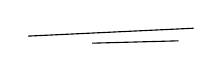
\begin{tikzpicture}\draw (0,0) -- (2.1,.10);\draw (.81,-.09) -- (1.91,-.06);\end{tikzpicture}}

\uline{Proposition} Let $G\xrightarrow{\deleted{\unsure{\lambda|v}}u}H$ \deleted{If} be a homomorphism of groups\deleted{, with $G$ quasi-compact} If $u$ is flat \inserted{(generizing)} at a point, it is flat \deleted{(at the \unsure{generic point})} \inserted{(\uline{universally} generizing)} \deleted{and \unsure{hence} \unsure{is} flat} ; \deleted{hence $u(G)$ stable under \deleted{specialization} generization.}

% slanted
\margin{An argument is needed for ``universally'' generizing.}
\deleted{\uline{Corollary} Suppose \deleted{that $H$ \unsure{quasi-compact} that there exists} that there exists a maximal point $x$ of $H$ such that $G_x\ne\varnothing$ (for example $u$ dominant and $G$ quasi-compact) Then \deleted{\unsure{$X$}} \inserted{if $H$ is reduced,} $u$ is flat, \deleted{hence generiz\unsure{ing} (hence generizing \ldots)} If one \inserted{does} not suppose \deleted{\uline{\unsure{Proposition}} Su} with $H$ reduced, $u$ is generizing, \deleted{and} the image \deleted{\unsure{of}} $u(H)$ is stable \inserted{in} under generization and \unsure{contains|contains}}

\uline{Corollary} Equivalent conditions on $u$

\deleted{\unsure{affine|open}} a) $u$ is \inserted{universally} generizing \quad---\quad a$'$) $u$ generizing at a point.

b) $\unsure{U(G)|u(G)}\supset \deleted{G}H_0$

c) $\exists$ a maximal point \inserted{$x$} of $G$ such that $u^{-1}(x)\ne\varnothing$.

Under these conditions, $u(G)$ is stable under specialization \deleted{(hence \unsure{closed if} $G$ quasi-compact)}\margin{\deleted{\unsure{and H locally of finite type}}}

\uline{Proof} a) $\Longrightarrow$ a$'$) known, a$'$) $\Longleftrightarrow$ b) \deleted{\illegible{1}} trivial, b) $\Longrightarrow$ c) trivial, let us prove c) $\longrightarrow$ b. Now $W=u(G)$ is stable \uline{under $\deleted{G}H_0$}, so the $\varphi_x$ being generizing, it is stable under specialization ; \deleted{OK} hence b) becomes trivial.

% slanted
\margin{\deleted{with} Is it \uline{always} true that $u(G)$ stable under specialization? Yes. I prove for every subset stable under multiplication (and inversion) $\to$ stable under specialization}
\uline{Corollary} If $G$ quasi-compact, \deleted{\unsure{dominance} of $H^{\unsure{\mathrm{red}|\mathrm{t}}}$ \unsure{over}} \inserted{$\operatorname{Im}u$ is closed}

\uline{Proposition.} If $G\longrightarrow H$ a monomorphism, with $G$, \deleted{$H$} of finite type, \inserted{$H$ locally of finite type} then $u$ is a closed immersion.

\figure{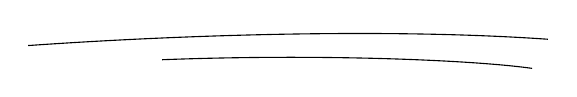
\begin{tikzpicture}\draw (0,0) .. controls (2,.14) and (4.6,.22) .. (6.6,.08);\draw (1.7,-.18) .. controls (3.8,-.10) and (5.7,-.19) .. (6.4,-.29);\end{tikzpicture}}

\diagram{$\displaystyle
\text{1)}\quad\left\{\begin{array}{l}
\text{Discrete groups (possibly twisted)}\\
\text{Groups profétales f. }(\text{---})\\
\text{Locally compact groups (totally disconnected) (possibly twisted}
\end{array}\right.
\quad\left|\begin{array}{l}
\text{groups}\\
\text{separable}\\
\text{totally disconnected}
\end{array}\right.$}

\[
\begin{aligned}
\underline{\approx}\quad &\text{locally compact topological groups}\\
 &\text{\inserted{totally disconnected} with \uline{continuous} actions of }\pi\\
 &\pi\times G\longrightarrow G\quad\text{continuous.}
\end{aligned}
\]

\diagram{$\displaystyle
\text{2)}\quad\begin{array}{l|l}
\text{\uline{Connected groups}} & \text{\uline{over a perfect field} : Extension (canonical)}\\
\text{\uline{\deleted{\unsure{s|S}}Separable}} & \text{of an abelian variety by a connected group}\\
\text{[are quasi-compact]} & \text{smooth affine}\quad\Longleftrightarrow\quad \underset{\longleftarrow}{\lim} G_i,\\
& \text{the }G_i\text{ of finite type, abelian part}\\
& \text{of bounded dimension.}
\end{array}$}
% archive sheet number: 5
